\chapter{Computational Study}

This chapter presents our computational study and is structured as follows: 
Section \ref{sec:data} describes the data our experiments are conducted on.
Section \ref{sec:samplesize} examines how different samples sizes used for training affect the test error.
In Section \ref{sec:hpo}, we optimize model hyperparameters and seek to get better intuition when for parameter configuration by analyzing parameters considered for our optimization.
Last but not least, section \ref{sec:noise} demonstrates how noise affects predictive performance of our models.

\section{Data exploration}\label{sec:data}
The available data set is provided by \cite{Hildebrandt2020_EAT} who created a high-dimensional data model with the RMDP instances originally used in \cite{UlmerRMDP}. It comprises 850.469 samples, 23.341 unique customer locations, a delivery fleet of 15 vehicles and 15 unique restaurant locations. The temporal and spatial distribution of the orders is depicted in figure \ref{fig:dists}. 
\begin{figure}[h]
	\centering
	\subfigure[Request arrival time distribution]{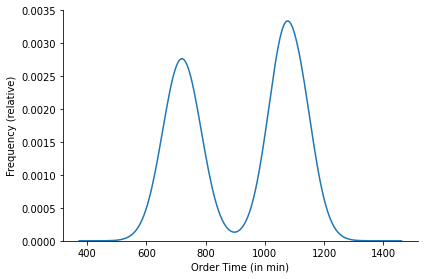
\includegraphics[width=0.49\linewidth]{../Implementation/DataDescription/order_time_dist.png}}
	\subfigure[Spatial distributions]{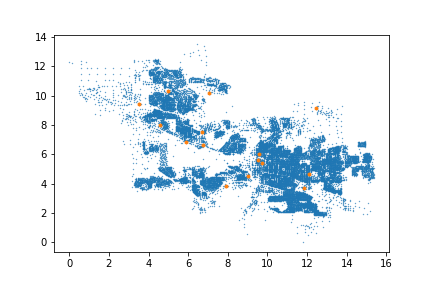
\includegraphics[width=0.49\linewidth]{../Implementation/DataDescription/spatial_dist.png}}
	\caption{Spatial and temporal distributions}
	\label{fig:dists}
\end{figure}

Panel (a) of figure \ref{fig:dists} shows the order behaviour of customers. The x-axis denotes the day time in minutes, the y-axis denotes the relative frequency of incoming customer orders for a given day time on the y-axis. We can observe that the order time behaviour across all customers follows a bimodal gaussian distribution. The order frequency peaks at around 12:00 a.m (roughly 700 minutes of day time) and again around 6.00 p.m (roughly 1100 minutes of day time). This indicates that the probability of an order taking place during lunch or dinner time is relatively high.  
Panel (b) of figure \ref{fig:dists} shows the spatial distribution of customer and restaurant locations. The x-axis depicts the  

\begin{figure}[h]
	\centering
	\subfigure[Delivery delay distribution]{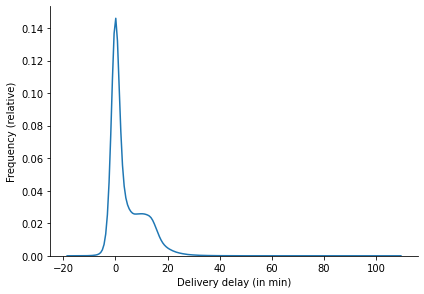
\includegraphics[width=0.49\linewidth]{../Implementation/DataDescription/delivery_delay.png}}
	\subfigure[Meal preparation time distribution]{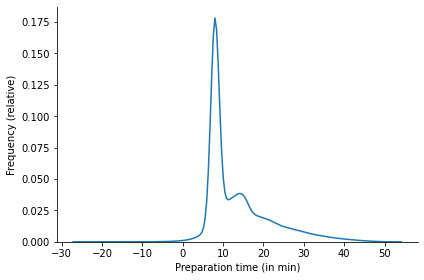
\includegraphics[width=0.49\linewidth]{../Implementation/DataDescription/prep_time.png}}
	\caption{Spatial and temporal distributions}
	\label{fig:prepdelay}
\end{figure}
Panel (a) of figure \ref{fig:prepdelay} shows the distribution of delivery delay times in minutes for all requests in the data. The delivery dela is here defined as the difference between actual and the expected time of arrival based on PoM. First, we observe that roughly 14-15\% of the requests in our data are delivered on time. Negative values for the delivery delay on the plot indicate that a rather tiny amount of orders happens to be delivered earlier than expected. However, we are most interested in the orders that are actually delivered later than expected. We observe that a non-trivial amount of orders is delivered with a delay of up to 20 minutes. As we will later show, arrival time estimation via supervised learning is a vastly better option compared to planning on means.
Since arrival times are impacted by uncertainty in meal preparation times, we take a look at their distribution in our data as well. In panel (b) of figure \ref{fig:prepdelay}, we observe that roughly a fifth of the orders had a preparation time of around 10 minutes. However, a non-trivial amount of orders seem to have quite longer preparation times ranging from 15 to less than 40 minutes. 

\section{Experiment: Different Sample Sizes}\label{sec:samplesize}

This section compares how a difference sample size impact the test error for each possible combination of models and datasets. With this experiment, we intend to examine how different sizes in training data affect the test error for the respective combination. Since less samples in the training data corresponds to lower training times, we use the results of this experiment for the subsequent hyperparameter optimization and the noise analysis to speed our experimental procedure up. For our linear model and the considered ensembles, we consider 100 training runs with every run corresponding to a sample subset size $ \{2000, 4000, \dots, 200.000\} $. For each model, we set the parameters manually since we did not conduct hyperparameter optimization yet. 

\begin{figure}[h]
	\centering
	\subfigure[For GBDT]{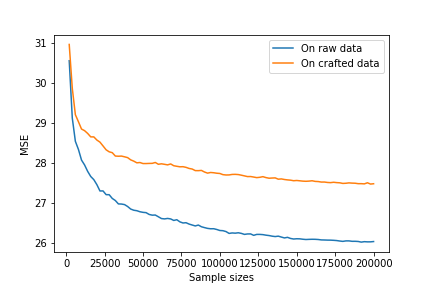
\includegraphics[width=0.49\linewidth]{../Implementation/SampleSize/GBDT_SampleSizes.png}}
	\subfigure[For Random Forest]{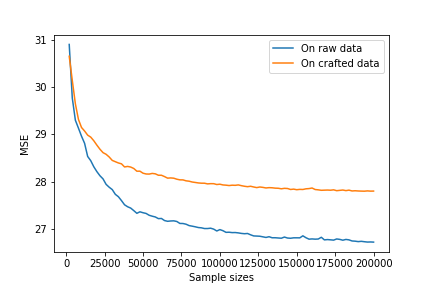
\includegraphics[width=0.49\linewidth]{../Implementation/SampleSize/RF_SampleSizes.png}}
	\subfigure[For Linear Regression]{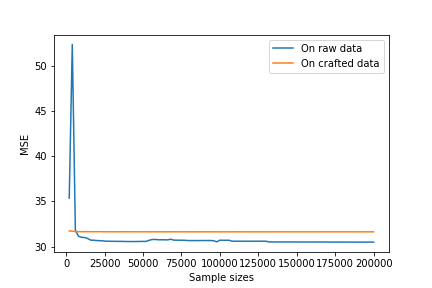
\includegraphics[width=0.49\linewidth]{../Implementation/SampleSize/LR_SampleSizes.png}}
	\caption{MSE for different sample sizes}
	\label{fig:prepdelay}
\end{figure}


\section{Experiment: Hyperparameter Optimization}\label{sec:hpo}
This section presents the hyperparameter optimization (HPO) experiments conducted for GBDTs, RFs, and the neural network. 
We use \textit{Optuna}, a popular HPO framework proposed and designed by \cite{akiba2019optuna}, to conduct our HPO experiments. 
\textit{Optuna} provides a simple implementation design that allows us to analyze several parameters of choice from different points of view. 
The optimizations were conducted on both the crafted data set and the raw data set. 
Concretely, we will proceed as follows: First, we will present the hyperparameters we decided to include in the HPO to then in turn present the optimal hyperparameter values resulting from the experiment and explore the predictive power of different parametrizations. 
For every GBDT and RF experiment instance, the hyperparameters will be sampled via the \textbf{C}ovariance \textbf{M}atrix \textbf{A}daption \textbf{E}volution \textbf{S}trategy, or in short \textbf{CMA-ES}. 
\textit{CMA-ES} follows a simple principle: The probability of samples from previously succesful optimization steps being drawn again is positively correlated to the contribution of those samples to the objective. For further information on \textit{CMA-ES}, the reader is referred to \cite{hansen2016cma}. 
To speed up the optimization process, we use the \textit{Optuna}-implementation of the \textit{Hyperband Pruner} presented in \cite{li2018hyperband}. 
By that, we hope to get a fine-tuned model that maximizes prediction quality on one hand, and intuition for parametrization on the other.
Secondly, we will use the \textit{optuna} implementation of the \textit{fANOVA} evaluation algorithm presented in \cite{fANOVA} to determine hyperparameter importances. 
In short, \textit{fANOVA} calculates feature importances by fitting a random forest regression model to the optimal parameter configuration that results of the HPO and predict the objective value with that model. For each parameter importance prediction, we set the number of estimators to 1000.
Thereby, we can assess which parameters impact the model significantly and which parameters are less significant, and especially how the importances differ for the two data sets. 
Lastly, we will examine interdependencies between the evaluated hyperparameters. 
 
\subsection{GBDT}

In this section, we will conduct HPO experiments for GBDTs on both datasets. 
For GBDT, we decided to optimize following parameters and set the search spaces for each them as follows:
\begin{description}[font=$\bullet$\scshape\bfseries]
	\item $ \text{learning\_rate} \in [0.01, 0.05] $  in steps of 0.001.
	\item $ \text{max\_depth} \in [5, 100] $ in steps of 0.001.
	\item $ \text{feature\_fraction} \in [0.1, 1.0] $ in steps of 0.01.
	\item $ \text{feature\_fraction\_bynode} \in [0.3, 1.0] $ in steps of 0.01
	\item $ \text{num\_leaves} \in [20, 300] $ in steps of 1
	\item $ \text{min\_child\_samples} \in [10, 400] $ in steps of 1.
	\item $ \text{subsample\_freq} \in [1, 10] $ in steps of 1.
	\item $ \text{subsample} \in [0.3, 1.0] $ in steps of 0.01.
\end{description}
Besides the parameters considered for optimization, we set the number of estimators for one iteration in GBDT to 1000 and enable early stopping with a patience of 50. Our selection of parameter search spaces is the result of trial-and-error since machine learning problems are highly individual and, as we have already demonstrated with our literature review, many different solution approaches are possible. The determination of parameter values respectively parameter search spaces therefore has to happen at least partly in a manual fashion, which is why we regard the trial-and-error heuristic as a suitable approach for the configuration of hyperparameter search spaces. Detailed descriptions of the considered parameters for the \textit{lightgbm}-GBDT implementation can be found under \url{https://lightgbm.readthedocs.io/en/latest/Parameters.html}.

Figure \ref{fig:GBDT_ParallelPlot} depicts the parameter configurations of each optimization epoch in form of a parallel coordinate plot for GBDT on raw data in panel (a) and on crafted data in panel (b). Except the vertical gray line one the very left in the plots, each vertical gray axis represents the values ranging within the defined intervall of its corresponding parameter, whereas the very left line represents the axis for the objective values. The lines connecting all the parameter axes represent the parameter configurations of the optimization epochs. The bluer a line, the better the objective value - in our case the mean squared error. 

At first glance, it can be seen directly that the parameter configurations of both plots for good predictive performance are quite similar. For both sets, the mean squared error is minimized when we roughly use two-thirds of the features for each GBDT iteration (feature\_fraction, feature\_fraction\_bynode). Less test error is achieved is more likely when we allow the algorithm to build rather deep trees (max\_depth) while constraining the tree splitting process by specifying a lower bound for the minimal amount of samples a node must contain in order to split it further (min\_child\_samples). We can furthermore see that a better objective value is attained when nearly all samples are used for a GBDT iteration (subsampling) and learning rates range between from 0.03 to 0.05 (learning\_rate).
Training GBDT with optimal parameter configuration using the full available amount of samples results in a mean squared test error of approximately 25.6780 on the raw data, and 27.0852 on the crafted data.
For the optimal parameter configurations for training GBDT on both data sets, the reader is referred to Appendix A.1 
%[TODO: Anhang.tex erstellen und Sachen einfügen]
\begin{figure}[h]
	\centering
	\subfigure[On raw data]{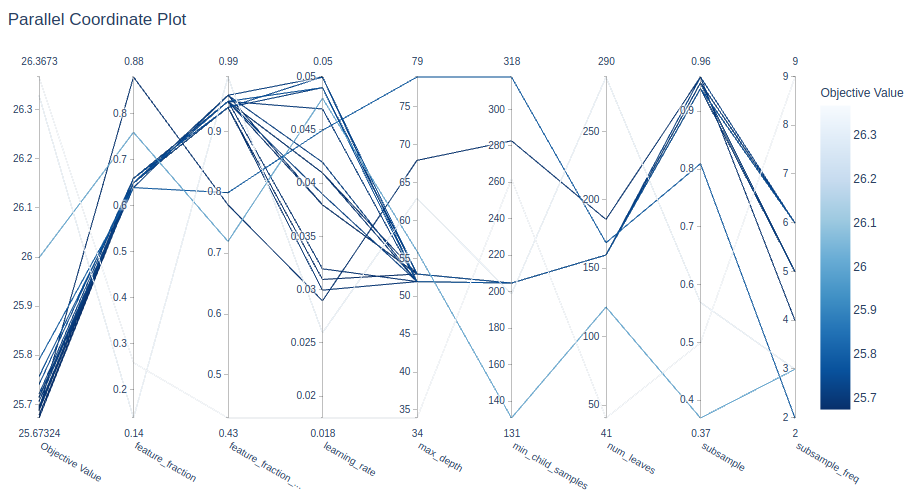
\includegraphics[width=\linewidth]{figures/HPO/GBDT_HPO_Raw_ParallelPlot.png}}
	\subfigure[On crafted data]{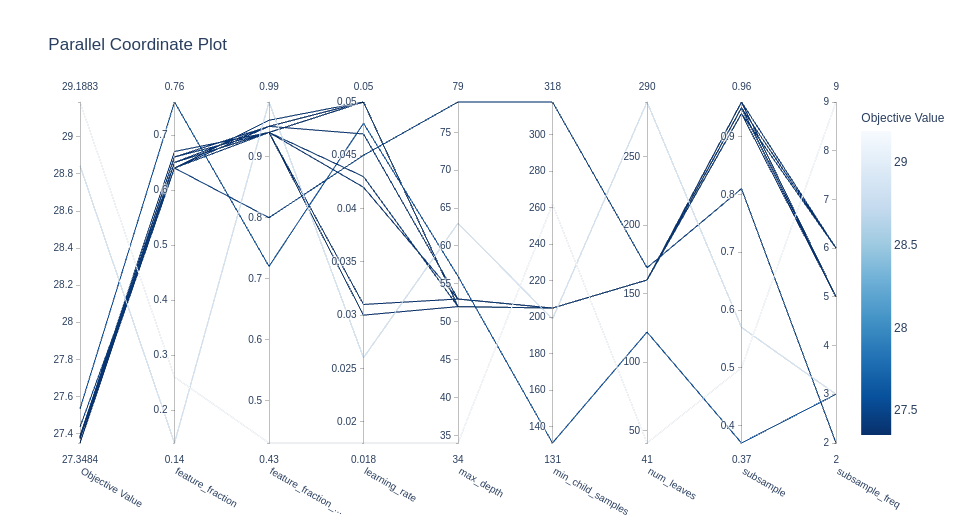
\includegraphics[width=\linewidth]{figures/HPO/GBDT_HPO_Crafted_ParallelPlot.png}}
	\caption{Parallel Coordinate Plots for GBDT}
	\label{fig:GBDT_ParallelPlot}
\end{figure}

Up next are the hyperparameter importances of GBDT depicted in figure \ref{fig:GBDT_Importances}. Panel (a) shows the importances for GBDT when trained on raw data. Panel (b) shows the importances for GBDT when trained on crafted data. The x-axis of the importance plots depicts the relative parameter importances. On the y-axis is categorical and shows the parameters we considered to optimize. We can observe that the results for the datasets GBDT was trained on differ significantly. For GBDT on the raw data, we observe that choosing the right amount for subsampling and a suitable learning rate for calculating the gradient in GBDT are of highest importance. We conclude that subsampling for all estimators seems to be counterintuitive with regards to our objective. Our parallel plot for GBDT on raw data in panel (a) of figure \ref{fig:GBDT_ParallelPlot}) also supports this claim, since most of the optimization epochs with subsample fraction values near to 1 are linked to lower objective values.
The right fraction of features to use for all estimators is highly interesting: While the feature fraction has a relative importance of 0.15 and is ranked third for GBDT on raw data as shown in panel (a), it is by far the most important hyperparameter when we train GBDT on our crafted data with a relative importance of 0.33. As a consequence of feature fraction being the most important hyperparameter on our crafted data, subsampling is pushed out of the first place and falls on the 4th rank with a relative importance of 0.10 and thus a decrease of 14\% when compared to GBDT on raw data. However, the learning rate maintains its relative importance of roughly 0.20 and its rank as the second most important parameter. We observe further non-trivial differences in relative importance for the subsampling frequency, the minimum amount of samples a child node has to have in order to be considered splitting. In both instances, the maximal depth constraint remains on the lowest ranks.
\begin{figure}[h]
	\centering
	\subfigure[On raw data]{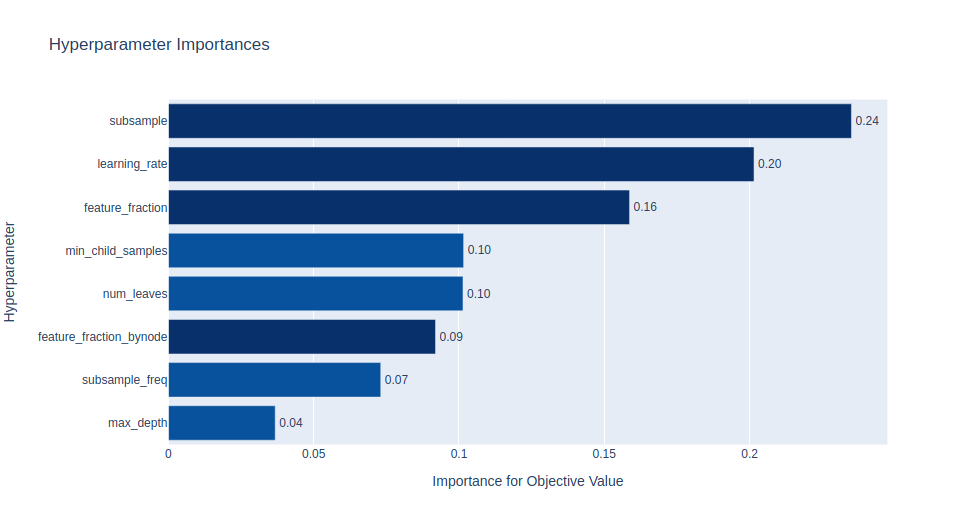
\includegraphics[width=\linewidth]{figures/HPO/GBDT_HPO_Raw_Importances.png}}
	\subfigure[On crafted data]{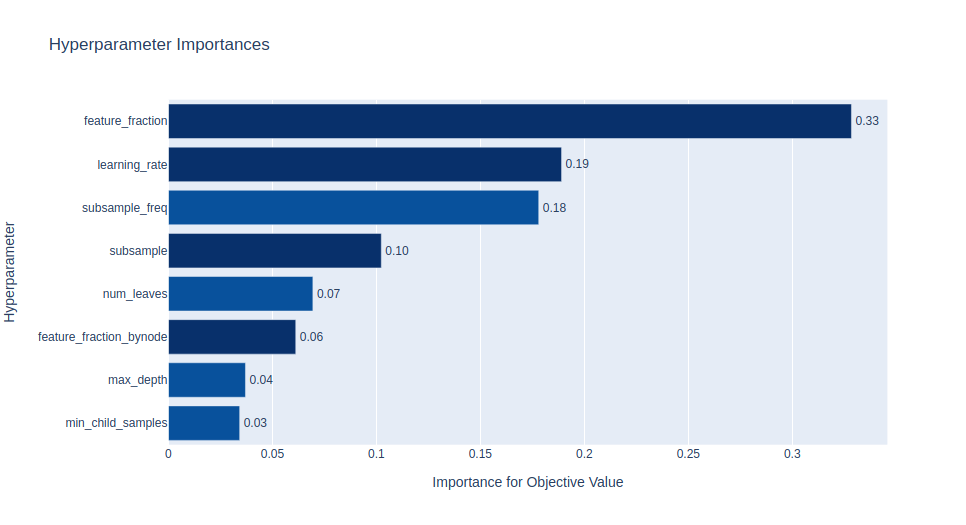
\includegraphics[width=\linewidth]{figures/HPO/GBDT_HPO_Crafted_Importances.png}}
	\caption{Hyperparameter Importances for GBDT}
	\label{fig:GBDT_Importances}
\end{figure}

\clearpage
\subsection{Random Forest}


\begin{figure}[h]
	\centering
	\subfigure[On raw data]{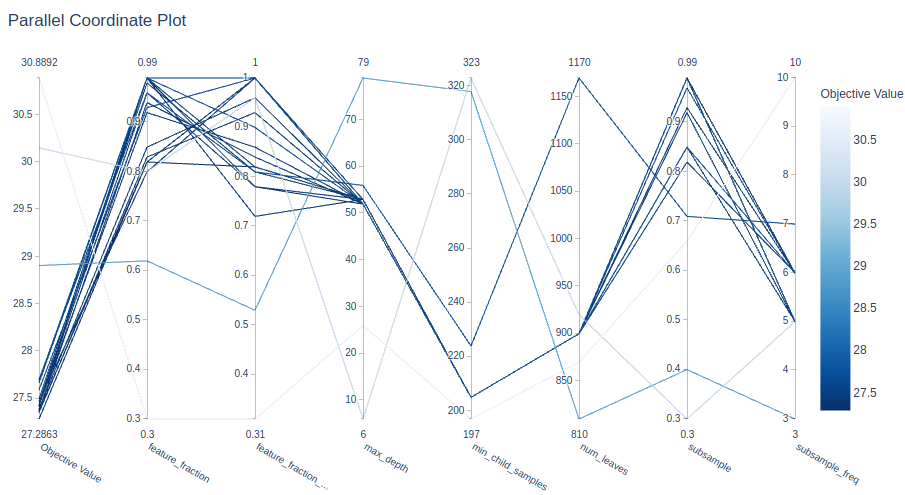
\includegraphics[width=\linewidth]{figures/HPO/RF_HPO_Raw_ParallelPlot.png}}
	\subfigure[On crafted data]{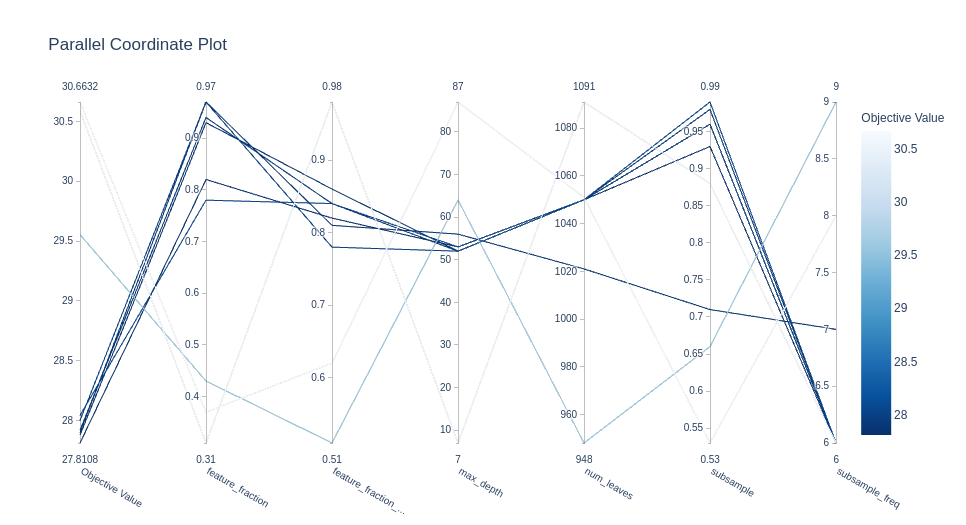
\includegraphics[width=\linewidth]{figures/HPO/RF_HPO_Crafted_ParallelPlot.png}}
	\caption{Parallel Coordinate Plots for Random Forest}
	\label{fig:RF_ParallelPlot}
\end{figure}
\begin{figure}[h]
	\centering
	\subfigure[On raw data]{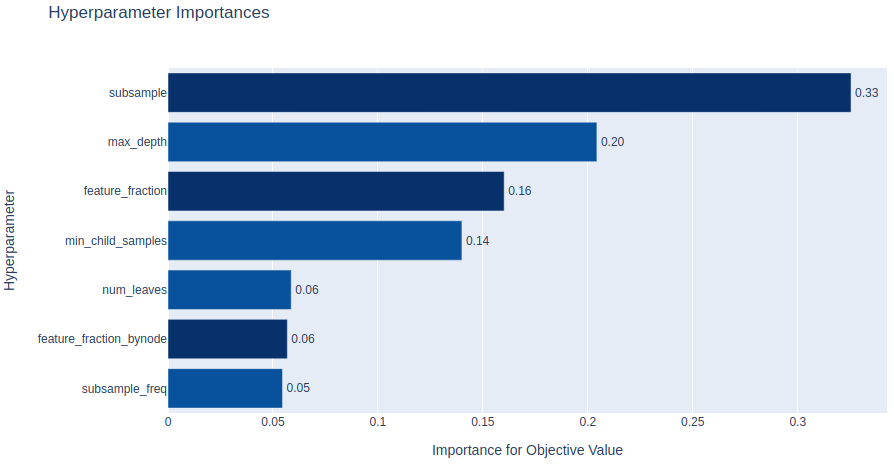
\includegraphics[width=\linewidth]{figures/HPO/RF_HPO_Raw_Importances.png}}
	\subfigure[On crafted data]{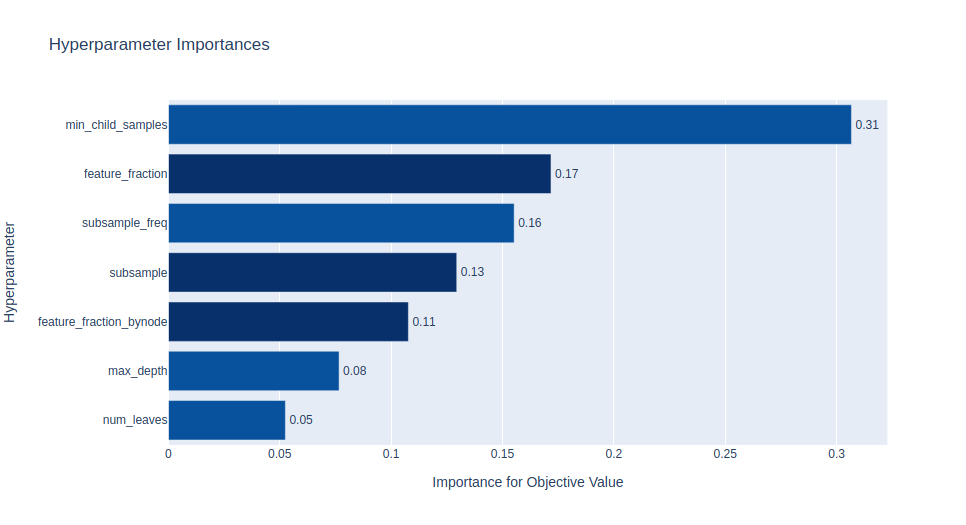
\includegraphics[width=\linewidth]{figures/HPO/RF_HPO_Crafted_Importances.png}}
	\caption{Hyperparameter Importances for GBDT}
	\label{fig:RF_Importances}
\end{figure} 

\section{Experiment: Adding Noise}\label{sec:noise}







